%
\documentclass[tikz, border=5pt]{standalone}
\usepackage{tikz}
\usepackage[dvipsnames]{xcolor}
\usetikzlibrary{calc, positioning}

\newcommand{\State}[2]{%
    % #1 : x
    % #2 : y
    \def\p{0.02} % Padding
    \begin{scope}
        \filldraw[fill=Blue!25]
        ($(#1,#2)+(-1+\p,0.5-\p)$)
        rectangle
        ($(#1,#2)+(1-\p,-0.5+\p)$);
        \node at (#1,#2) {State};
    \end{scope}
}

\newcommand{\Action}[2]{%
    % #1 : x
    % #2 : y
    \begin{scope}
        \filldraw[fill=Green!25]
        ($(#1,#2)+(-1+\p,0.5-\p)$)
        rectangle
        ($(#1,#2)+(1-\p,-0.5+\p)$);
        \node at (#1,#2) {Action};
    \end{scope}
}

\begin{document}
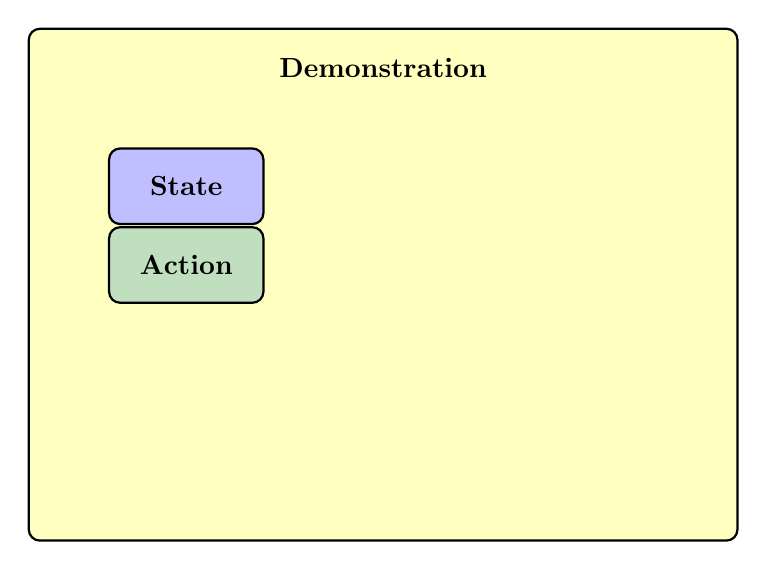
\begin{tikzpicture}[
        thick,
        draw=black,
        rounded corners,
        font=\bfseries,
    ]

    \def\xleft{0}
    \def\xright{9}
    \def\ytop{0}
    \def\ybottom{-6.5}
    \def\h{1.75}

    \pgfmathsetmacro{\xmid}{(\xleft+\xright)/2}
    \pgfmathsetmacro{\ymid}{(\ytop+\ybottom)/2}

    \filldraw[fill=Yellow!25]
    (\xleft,\ytop) rectangle (\xright,\ybottom);
    \node at (\xmid,\ytop-0.5) {Demonstration};

    \State{2}{-2};
    \Action{2}{-3};

\end{tikzpicture}
\end{document}
